\chapter{Weryfikacja modelowa}

Systemy tworzone przez ludzi są coraz bardziej złożone oraz odgrywają coraz większą rolę w życiu każdego z nas.
Błędy w oprogramowaniu skutkują stratami finansowymi, wizerunkowymi, opóźnieniami, a także utratą zdrowia i życia ludzi. Dowodzą temu następujące przykłady: nieudany start Ariane-5 (04.06.1996), błąd w procesorach Pentium II Intela, czy źle działająca maszyna do radioterapii spowodowała śmierć sześciu pacjentów w latach 1985-1987.


\section{Weryfikacja systemu}

Weryfikacja systemu ma na celu ustalenie, czy projekt posiada oczekiwane właściwości. Mogą one być dość podstawowe, np. nigdy nie dojdzie do zakleszczenia lub związane z domeną, np. nie można wypłacić więcej pieniędzy, niż jest na koncie. Specyfikacja dostarcza informacji, jak system może oraz jak nie może się zachowywać. Oprogramowanie uważa się za poprawne, jeśli spełnia wszystkie właściwości. Schemat weryfikacji został przedstawiony na rys. \ref{fig:system_verification_scheme}.

\begin{figure}[h]
    \centering
    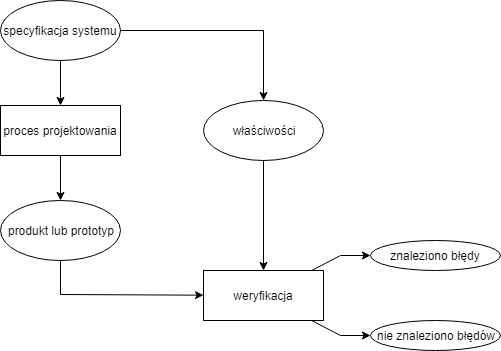
\includegraphics[height=8cm,keepaspectratio]{img/system_verification_schematic_view.png}
    \caption{Schemat tworzenia systemu wraz z jego weryfikacją (źródło~\cite{Bai08}).}
    \label{fig:system_verification_scheme}
\end{figure}

Podstawową formą radzenia sobie z tym problemem jest testowanie oprogramowania (testy jednostkowe, integracyjne, systemowe itp.). Polega to na uruchamianiu kodu dla różnych ścieżek wykonania, po czym porównuje się ich wyjścia z oczekiwanymi. Niestety, przetestowanie wszystkiego okazuje się praktycznie niemożliwe, zwykle sprawdzane są jedynie warunki brzegowe (stanowi to mały podzbiór wszystkich kombinacji). 


\section{Weryfikacja modelowa}

Podczas tworzenia skomplikowanych systemów, kładzie się coraz większy nacisk na testowanie poprawności oprogramowania. Metody formalne mają duży potencjał na tym polu. Ich wczesna integracja (podczas procesu projektowania) dostarcza efektywnych technik weryfikacji.
Intuicyjnie, metody formalne można rozważać jako matematykę stosowaną dla modelowania i analizy systemów informatycznych. Zapewniają one poprawność z matematyczną dokładnością.

Techniki weryfikacji bazujące na modelu opisują zachowanie systemu deterministycznie i kompletnie. Samo tworzenie pełnego modelu może wykryć luki lub niespójności.
Po jego stworzeniu, wraz z otaczającymi algorytmami, możliwe jest eksplorowanie stanów systemu.
Dzieje się to w podejściu "brute-force" - przejrzane zostają wszystkie możliwe scenariusze.
W ten sposób udowadnia się spełnialność właściwości. Możliwa jest również weryfikacja powiązana z czasem, np. czy system zawsze odpowie poniżej oczekiwanych 5 sekund.

\begin{figure}[h]
    \centering
    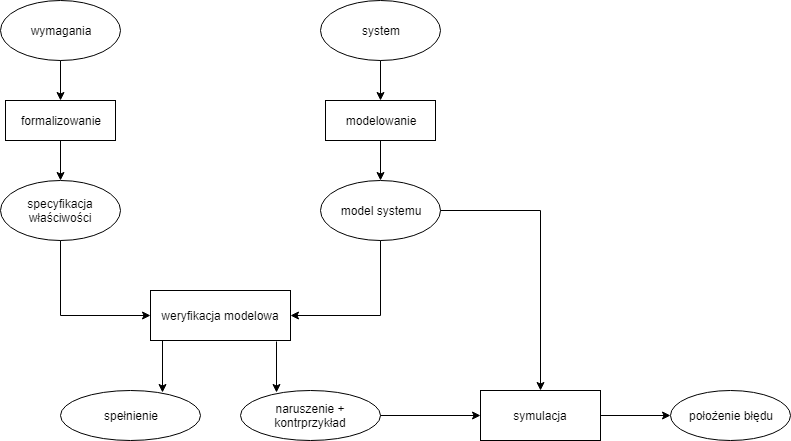
\includegraphics[width=\textwidth,keepaspectratio]{img/model_checking_approach_schematic_view.png}
    \caption{Schemat podejścia weryfikacji modelowej (źródło~\cite{Bai08}).}
    \label{fig:model_checking_scheme}
\end{figure}

Podejście to świetnie sprawdza się w wykrywaniu (częstych) błędów związanych z wielowątkowością. Typowe oczekiwane właściwości:
\begin{itemize}
\item osiągalność (niemożliwe jest zakleszczenie)
\item bezpieczeństwo (coś niepożądanego nigdy nie wystąpi \cite{Alp87})
\item żywotność (coś "dobrego" w końcu nastąpi \cite{Alp85})
\item uczciwość (czy przy odpowiednich warunkach zdarzenie występuje powtarzalnie)
\item właściwości czasu rzeczywistego
\end{itemize}

\vspace{0.5cm}
Model systemu zazwyczaj generuje się automatycznie z opisu w odpowiednim języku lub dialekcie wspieranym przez narzędzie. 
Weryfikator modelowy przeszukuje kolejne stany. Następnie sprawdzane są pod kątem właściwości. Po znalezieniu naruszenia, prezentowany zostaje kontrprzykład wraz z całą ścieżką wykonania, która do niego prowadzi. Pozwala to łatwo odtworzyć całą ścieżkę, a także znaleźć niespójność, która wymaga zmiany modelu (lub właściwości) - schemat na rys. \ref{fig:model_checking_scheme}.

\vspace{0.5cm}
\noindent
To nie jedyne zalety, kolejnymi mocnymi stronami weryfikacji modelowej są:
\begin{itemize}
\item To ogólna metoda weryfikacji, która sprawdza się zarówno przy tworzeniu oprogramowania, jak i projektowaniu sprzętu (np. procesorów).
\item Wspiera częściową weryfikację - możemy sprawdzać poszczególne właściwości niezależnie, nawet gdy pełna specyfikacja nie jest gotowa.
\item Wszystkie możliwości zostają sprawdzone.
\item Dostarcza informacji diagnostycznych po wykryciu niespełnionej właściwości.
\item Uruchomienie weryfikatora nie wymaga ekspertyzy na tym polu.
\item Łatwo zintegrować to rozwiązanie z cyklem wytwarzania oprogramowania.
\item Obecnie wzrasta zainteresowania tym podejściem.
\end{itemize}

\vspace{0.5cm}
\noindent
Oczywiście nie brak także wad:
\begin{itemize}
\item Weryfikowany jest model systemu, a nie sam system. Brak tu gwarancji, że implementacja poprawnie go odtwarza.
\item Sprawdzane są tylko wykorzystane wymagania. Nie można wnioskować o poprawności właściwości, które nie zostały sprawdzone (błąd niedokładnej specyfikacji \cite{Lam05}).
\item Aplikacje oparte na dużej ilości danych mogą posiadać zbyt wiele stanów, aby je wszystkie wygenerować, a nawet ich liczba może być nieskończona.
\item Podatność na problem eksplozji przestrzeni stanów \cite{Cla11}.
\end{itemize}


\section{Logika LTL}

Logika LTL to jednak z logik temporalnych. Opiera się na liniowej strukturze czasu.
Jej składnia i semantyka pozwala precyzyjnie opisywać właściwości systemu.
"Temporalna" oznacza umiejscawianie zdarzeń relatywnie względem innych, to pewna abstrakcja ponad czasem.  Z tego powodu niewykonalne jest sprawdzenie, czy maksymalne opóźnienie między zdarzeniami wynosi $500ms$.

Składnia LTL
- spis skladni, Intuitive semantics of temporal modali (obrazek)

\begin{figure}[h]
    \centering
    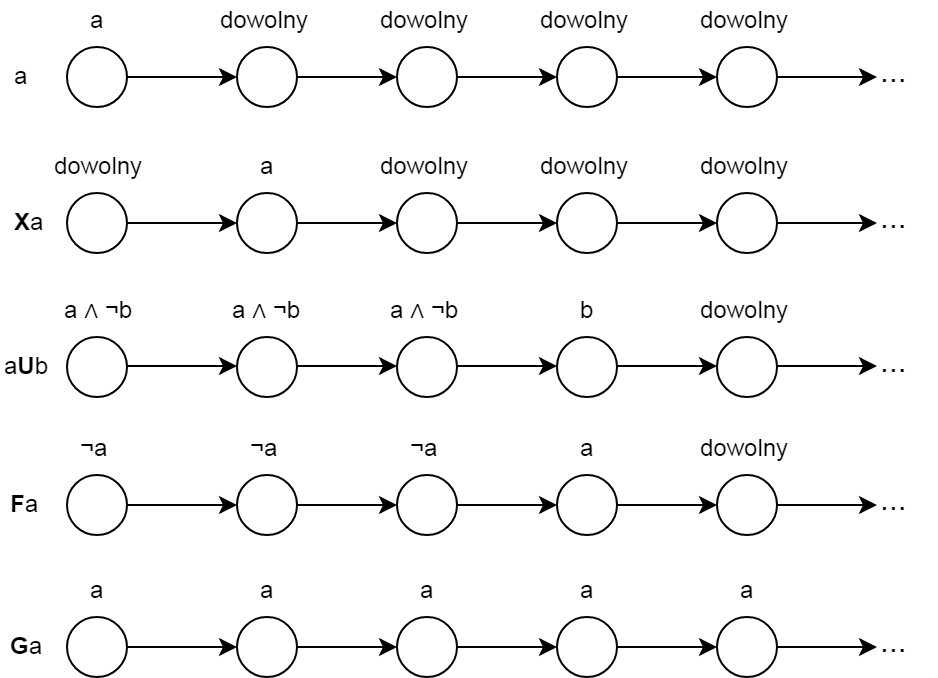
\includegraphics[width=\textwidth,keepaspectratio]{img/ltl_intuitive_semantics.png}
    \caption{Intuicyjna semantyka temporalnych modalności (źródło~\cite{Bai08}).}
    \label{fig:ltl_semantics}
\end{figure}


\section{Ignore}

TODO

weryfikacja modelowa, przestrzen stanow, LTL (co to, opis skladni, operatorow, przyklad z opisem), automaty, automaty buchiego (przykladowe obrazki automatow z podanej formuly LTL, opis ze potrzebna negacja i szukanie spelnialnosci)
weryfikacja hardware i software
alogrytmy wykorzystywane w przeszukiwaniu i weryfikacji
co to i po co on-the-fly
Alvis, co to, po co

\cite{Bar12} \cite{Jac05}
przejrzec publikacje profesora


w czesci implementacji:
opis weryfikowanego systemu


A time-optimal on-the-fly parallel algorithm for model checking of weak LTL properties, in: Formal Methods and Software Engineering

 
